\documentclass{Arquivos/AbnTexUFT}

\titulo{Modelo \abnTexUFT para\\ Relatório Técnico por \WenesTex}
\autor{Editado por \WenesTex Aquino}

\orientador{Fulano Aquino Carvalho}
\coorientador{Beltrano Vitória Almeida}

\local{Palmas}
\data{2025, v-1.2}

\instituicao{%
  Universidade Federal do Tocantins \\
  Campus Universitário de Palmas \\
  Curso de Licenciatura em Computação
}

\preambulo{Relatório Técnico apresentado como 
    parte dos requisitos para avaliação na Universidade 
    Federal do Tocantins. Este modelo foi adaptado 
    e personalizado com ajustes visuais e estruturais, 
    servindo também para testar o espaço disponível 
    utilizada nessa contracapa.}


% =======================================================================================================================
% INÍCIO DO DOCUMENTO
% =======================================================================================================================
\begin{document}
\nocite{*} 



% -----------------------------------------------
% ----------FOLHA DE ROSTO E CONTRACAPA----------
% -----------------------------------------------
\imprimircapa         % Está é Folha de Rosto
% -----------------------------------------------
\imprimirfolhaderosto % Esta é Contracapa
% -----------------------------------------------







% ============================================
\chapterstyle{default} 
\setlength{\beforechapskip}{-1.5cm} % Distancia entre Capitulo e Top
\setlength{\afterchapskip}{1.5cm}   % Espaço entre o título e o texto
% ============================================








% ============================================
% --- Agradecimentos ---
% ============================================
\tituloPreTextual{Agradecimentos}
\lipsum[101-102]




% ============================================
% --- Resumo em Português ---
% ============================================
\tituloPreTextual{Resumo}
\noindent Como afirma \cite{linux2024} \lipsum[1]

% ============================================
% --- Resumo em Inglês ---
% ============================================
\tituloPreTextual{Abstract}
\noindent \lipsum[1]
\clearpage





% -----------------------------------------------
% -----------------ILUSTRAÇÕES-------------------
% -----------------------------------------------
\pdfbookmark[0]{\listfigurename}{lof}
\listoffigures*
\thispagestyle{empty}
\cleardoublepage
% -----------------------------------------------


% -----------------------------------------------
% ------------------TABELAS----------------------
% -----------------------------------------------
\pdfbookmark[0]{\listtablename}{lot}
\listoftables*
\thispagestyle{empty}
\cleardoublepage
% -----------------------------------------------







% ============================================
% --- Sumário (SEM NÚMERO NENHUM) ---
% ============================================
\clearpage
% 1. Desliga cabeçalhos e rodapés gerais
\pagestyle{empty} 

% 2. Força a primeira página do sumário (que é um capítulo) a ser vazia também
\aliaspagestyle{chapter}{empty} 

\tableofcontents* \cleardoublepage

% Volta a primeira página dos capítulos a ter número (plain)
\aliaspagestyle{chapter}{plain} 
% Volta o estilo geral (meuestilo)
\pagestyle{meuestilo} 
% ============================================




% ============================================
% --- Limpeza e Início do Texto ---
% ============================================
\clearpage
\makeevenfoot{meuestilo}{}{}{} 
\makeoddfoot{meuestilo}{}{}{}  
\makeevenfoot{plain}{}{}{}
\makeoddfoot{plain}{}{}{}
\pagestyle{meuestilo}
% ============================================





% ============================================
% ELEMENTOS TEXTUAIS
% ============================================
\capituloNaoNumerado{Introdução}
\lipsum[1]
\chapterstyle{CapituloEstiloso} % Ativa Capitulo Estiloso



\part{Preparação}


\chapter{Justificativa}
\section{Coleta de Dados}
\lipsum[5]



\begin{figure}[h]
    \centering
    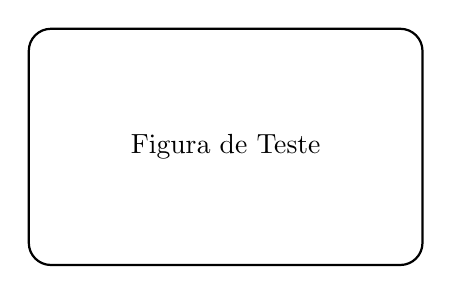
\begin{tikzpicture}
        \draw[rounded corners=8pt, thick] (0,0) rectangle (5,3);
        \node at (2.5,1.5) {Figura de Teste};
    \end{tikzpicture}
    \caption{Figura de teste estilizada}
    \label{fig:teste-estilosa}
\end{figure}



\begin{table}[h]
    \centering
    \label{tab:estilosa}
    \begin{tabular}{ccccc}
        \toprule
        Col 1 & Col 2 & Col 3 & Col 4 & Col 5 \\
        \midrule
        A1 & B1 & C1 & D1 & E1 \\
        A2 & B2 & C2 & D2 & E2 \\
        A3 & B3 & C3 & D3 & E3 \\
        A4 & B4 & C4 & D4 & E4 \\
        A5 & B5 & C5 & D5 & E5 \\
        \bottomrule
    \end{tabular}
    \caption{Tabela estilosa 5×5}
\end{table}




\section{Maecenas eget}
\lipsum[55]

\chapter{Metodologia}
\section{Praesent vel arcu}
\lipsum[5]

\section{Donec pellentesque}
\lipsum[55]

\part{Resultados}

\chapter{Análise}
\section{Nullam lacinia}
\lipsum[5]

\section{Maecenas eget}
\lipsum[55]

\chapter{Teste de Titulos Grandes - Análise vertical e horizontal: conceito, diferenças e cálculos Matemáticos}
\section{Fusce facilisis lacinia}
\lipsum[5]

\section{Maecenas eget}
\lipsum[55]


% --- RESPIRO ANTES DA CONCLUSÃO ---
\addtocontents{toc}{\protect\addvspace{1em}}
\chapter{Conclusão}
\lipsum[77]


% ============================================
% --- REFERENCIAS ---
% ============================================
\printbibliography[heading=referencias_abnt]
\clearpage
% ============================================



% ============================================
% --- APÊNDICES ---
% ============================================
\appendix
\paginaDivisoria{APÊNDICES}

\chapter{Entrevistas}
\section{Quisque ullamcorper placerat}
\lipsum[4]
\section{Quisque libero justo}
\lipsum[9]

\chapter{Roteiro de Entrevistas}
\section{Quisque ullamcorper placerat}
\lipsum[4]
\section{Quisque libero justo}
\lipsum[9]
% ============================================



% ============================================
% --- ANEXOS ---
% ============================================
\iniciarAnexos
\paginaDivisoria{ANEXOS}

\chapter{Mapa da Cidade}
\lipsum[2]
\section{Vivamus eu tellus}
\lipsum[1]
\section{Nam quis enim}
\lipsum[101]

\chapter{Mapa da Cidade}
\section{Vivamus eu tellus}
\lipsum[1]
\section{Nam quis enim}
\lipsum[101]
% ============================================

\end{document} 